\documentclass[a4 paper,12pt]{article}
\usepackage[inner=2.0cm,outer=2.0cm,top=2.0cm,bottom=2.0cm]{geometry}
\linespread{1.1}
\usepackage{setspace}
\usepackage[rgb]{xcolor}
\usepackage{verbatim}
\usepackage{subcaption}
\usepackage{longtable}
\usepackage{fancyhdr}
\usepackage{fullpage}
\usepackage[colorlinks=true, urlcolor=blue, linkcolor=blue, citecolor=blue]{hyperref}
\usepackage{booktabs}
\usepackage{amsmath,amsfonts,amsthm,amssymb}
\usepackage[shortlabels]{enumitem}
\usepackage{setspace}
\usepackage{extramarks}
\usepackage{soul,color}
\usepackage{graphicx,float,wrapfig}
\usepackage{tikz}
\usepackage{pgfplots}
\usepackage{amsmath}

\newenvironment{breakablealgorithm}
  {% \begin{breakablealgorithm}
   \begin{center}
     \refstepcounter{algorithm}% New algorithm
     \hrule height.8pt depth0pt \kern2pt% \@fs@pre for \@fs@ruled
     \renewcommand{\caption}[2][\relax]{% Make a new \caption
       {\raggedright\textbf{\ALG@name~\thealgorithm} ##2\par}%
       \ifx\relax##1\relax % #1 is \relax
         \addcontentsline{loa}{algorithm}{\protect\numberline{\thealgorithm}##2}%
       \else % #1 is not \relax
         \addcontentsline{loa}{algorithm}{\protect\numberline{\thealgorithm}##1}%
       \fi
       \kern2pt\hrule\kern2pt
     }
  }{% \end{breakablealgorithm}
     \kern2pt\hrule\relax%
   \end{center}
  }
\makeatother
\newtheoremstyle{definitionstyle}
  {3pt} % Space above
  {3pt} % Space below
  {\normalfont} % Body font
  {} % Indent amount
  {\bfseries} % Theorem head font
  {} % Punctuation after theorem head
  { } % Space after theorem head
  {} % Theorem head spec (can be left empty, meaning `normal`)

\theoremstyle{definitionstyle}
\newtheorem{defn}{Definition}
\newtheorem{thm}{Theorem}
\newtheorem{lem}{Lemma}
\newtheorem{statement}{Statement}
% \newtheorem{proof}{Proof}
\usepackage{framed}
\newenvironment{framedminipage}
    {\begin{framed}\begin{minipage}{0.9\textwidth}}
    {\end{minipage}\end{framed}}
\newcommand{\homework}[3]{
	\pagestyle{myheadings}
	\thispagestyle{plain}
	\newpage
	\setcounter{page}{1}
	\noindent
	\begin{center}
		\framebox{
			\vbox{\vspace{2mm}
				\hbox to 6.28in { {\bf Deep Learning \hfill} {\hfill {\rm #2} {\rm #3}} }
				\vspace{4mm}
				\hbox to 6.28in { {\Large \hfill #1  \hfill} }
				\vspace{3mm}}
		}
	\end{center}
	\vspace*{4mm}
}
\newcommand\numberthis{\addtocounter{equation}{1}\tag{\theequation}}

\begin{document}
\homework{CP2 Report}{2024011303}{Liu Hanzuo}
\section*{Training Techniques}
\paragraph{Model Structure}: from \texttt{Dropout} to \texttt{NoDropout} models, I only remove the dropout layers in the convolution layers. Which is mentioned in class -- a dropout layer should not follows a BatchNorm layer. \\
From \texttt{Vgg} models to other models, I add residual connection layers, using a "same" padding and a kernel size of 3 (like DenseNet), leading to a roughly 1\% improvement. (Since the model is not deep enough, the residual connection does not have a significant improvement.).\\
From \texttt{Deep} models to \texttt{Dropout} models, I change the connection ways: In the \texttt{Deep} architecture, there are 2 Resnets between convs: res1 and res2, the shedule is like:
\[
    x\to y=res1(x)+x\to res2(y)+y
\]
However, this structure does not works well due to limited model size. Thus I change the structure to:
\[
    x\to y=\text{cat}[res1(x),res2(x)]
\]
To describe it simply, the model's width also means much when the model's size is limited.\\
Moreover, I use a linear layer for last several layer's result (such as project them to a 32/64-dimension space), after concat them, we finally use a linear layer to get the final result. After checking this idea in CNN-relative papers, I find out that this idea is similar to ResNeXt, which improve the model's performance for about 1\%.\\
Finally, I change the structure of residual connection: instead of using residual connection between each two layers, I put the sum of all previous layers' result to the final layer. This structure is similar to DenseNet, which could extract each range of features in the photo. (the specific structure is showed afterwards)\\
\paragraph{Data Augmentation}:
The following data augmentation techniques were applied during training to improve the model's robustness and performance:
\begin{itemize}
    \item \textbf{Random Horizontal Flip}: Randomly flips the image horizontally.
    \item \textbf{Random Crop}: Crops the image to 128x128 pixels with a padding of 4 pixels.
    \item \textbf{Random Rotation}: Rotates the image by a random angle up to 30 degrees.
    \item \textbf{Color Jitter}: Randomly changes the brightness, contrast, saturation, and hue of the image.
    \item \textbf{Random Grayscale}: Converts the image to grayscale with a probability of 0.2.
    \item \textbf{Random Affine}: Applies random affine transformations with translation up to 25\% of the image size.
    \item \textbf{Random Perspective}: Applies random perspective transformations with a distortion scale of 0.3 and a probability of 0.5.
    \item \textbf{Normalization}: Normalizes the image with mean [125/255, 124/255, 115/255] and standard deviation [60/255, 59/255, 64/255].
    \item \textbf{MixUp}: Use torchvision's MixUp augmentation with a alpha of 0.1$\to$0.5.
\end{itemize}
In fact, data augmentation is a good way to prevent model from overfitting. However, the model's size is limited, thus the data augmentation could not be setted too hard (like RandomResizedCrop, RandomPerspective, etc.). Otherwise, the model will not converge. These parameters are setted after several tries.
\section*{Specific Model structures}
\paragraph{ResBlock}
\begin{verbatim}
def createManyResBlock(self, channels=64, BlockNum=3, kernel_size=3):
    self.cnt += 1
    manyResBlock = []
    for i in range(BlockNum):
        x = nn.Sequential(
            nn.Conv2d(channels, channels, kernel_size, padding=(kernel_size-1)//2),
            nn.BatchNorm2d(channels),
            nn.SiLU(),
            nn.Dropout2d(0.15 if channels < 128 else 0.25),
            nn.Conv2d(channels, channels, kernel_size, padding=(kernel_size-1)//2),
        )
        self.add_module(f'{self.cnt}_{i}', x)
        manyResBlock.append(x)
    return manyResBlock

def PassThrough(self, manyResBlock: list, x):
    for i in range(len(manyResBlock)):
        x = F.mish(x + manyResBlock[i](x))
        if i % 2:
            x = nn.Dropout2d(0.1)(x)
    return x
\end{verbatim}
\paragraph{ResBlock-Modified}
\begin{verbatim}
    def createManyResBlock(self, channels=64, BlockNum=3, kernel_size=3):
    self.cnt += 1
    manyResBlock = []
    for i in range(BlockNum):
        x = nn.Sequential(
            nn.Conv2d(channels, channels, kernel_size, padding=(kernel_size-1)//2),
            nn.BatchNorm2d(channels),
            nn.SiLU(),
            nn.Conv2d(channels, channels, kernel_size, padding=(kernel_size-1)//2),
        )
        self.add_module(f'{self.cnt}_{i}', x)
        manyResBlock.append(x)
    return manyResBlock

def PassThrough(self, manyResBlock: list, x):
    sequence = [ x ]
    for i in range(len(manyResBlock)):
        for j in range(i):
            x = F.mish(x + sequence[j])
        x = F.mish(x + manyResBlock[i](x))
        sequence.append(x)
    return x
\end{verbatim}
Here we show the ResBlock structure. The ResBlock is a basic block in the model. It is a combination of two convolution layers, with a BatchNorm layer and a SiLU activation layer. The dropout layer is added after the first. In the model architecture, we only change the hyperparameter in the function.
\paragraph{Model Architecture}
Notation: In the following graph, here are some definitions.
\begin{enumerate}
    \item inc: input channels, outc: output channels, c: channels in ResBlock, ks: kernel size, ps: padding size, s: stride size
    \item bn: block number, dr: dropout rate
    \item Concat: Concatenate the two inputs, ResConnect: enumerate before, pass the input through Resblocks consequently.
\end{enumerate}
\begin{longtable}{|c|c|c|c|c|}
    \caption{Model Architecture Layers} \label{tab:model_architecture} \\
    \hline
    \textbf{Layers} & \textbf{Basic Configs} & \textbf{Deep} & \textbf{Dropout} & \textbf{NoDropout-concat} \\
    \hline
    \endfirsthead
    \multicolumn{5}{c}{{\bfseries \tablename\ \thetable{} -- continued from previous page}} \\
    \hline
    \textbf{Layers} & \textbf{Basic Configs} & \textbf{Deep} & \textbf{Dropout} & \textbf{NoDropout} \\
    \hline
    \endhead
    \hline \multicolumn{5}{|r|}{{Continued on next page}} \\ \hline
    \endfoot
    \hline
    \endlastfoot
    Conv1 & inc=3, outc=64, ks=7, ps=3  & & & \\
    BatchNorm & c=64 & & & \\
    Maxpool & ks=2 & & & \\
    Dropout & dr=0.15 & & & dr=0.0\\
    \hline
    ResBlock11 & c=64, ks=3, bn=3 & & & \\
    ResBlock12 & c=64, ks=5, bn=3 & ks=3 & & \\
    Connection & & ResConnect & Concat & Concat\\
    \hline
    Conv2 & inc=outc=128, ks=3, ps=1, s=2 & & & \\      
    BatchNorm & c=128 & & & \\
    Maxpool & ks=2 & & & \\
    Dropout & dr=0.25 & & & dr=0.0\\
    \hline
    ResBlock2 & c=128, ks=3, bn=5 & & & \\
    \hline
    Conv3 & inc=128, outc=128, ks=5, ps=2 & & & \\
    BatchNorm & c=128 & & & \\
    Maxpool & ks=2 & & & \\
    Dropout & dr=0.25 & & & dr=0.0\\
    Linear1 & outc=32 & x & x & \\
    \hline
    ResBlock3 & c=128, ks=3, ps=1 & & & \\
    Linear2 & outc=32 & x & x & \\
    \hline
    Conv4 & inc=128, outc=64, ks=3, ps=1 & & & \\
    BatchNorm & c=64 & & & \\
    Maxpool & ks=2 & & & \\
    Dropout & dr=0.25 & & & dr=0.0\\
    Linear3 & outc=64 & x & x & \\
    \hline
    ResBlock4 & c=64, ks=3, ps=1 & & & \\
    Linear4 & outc=64 & x & x & \\
    \hline
    AvgPool & ks=4 & & & \\
    Linear5 & outc=64 & x & x & \\
    \hline
    Concat Linear & x & x & x & \\
    \hline
    Linear & inc=64, outc=256 & & & inc=256 \\
    BatchNorm & c=256 & & & \\
    GELU & & & & \\
    Dropout & dr=0.3 & & & \\
    Linear & inc=256, outc=256 & & & \\
    BatchNorm & c=256 & & & \\
    GELU & & & & \\
    Dropout & dr=0.2 & & & \\
    Linear & inc=256, outc=10 & & & \\      
    \hline
\end{longtable}
\section*{Training Curves}
\begin{figure}[H]
    \centering
    \begin{minipage}{0.48\textwidth}
        \centering
        \includegraphics[width=\textwidth]{train_loss.png}
        \caption{Training Loss Curve}
        \label{fig:train_loss}
    \end{minipage}
    \hfill
    \begin{minipage}{0.48\textwidth}
        \centering
        \includegraphics[width=\textwidth]{train_accuracy.png}
        \caption{Training Accuracy Curve}
        \label{fig:train_accuracy}
    \end{minipage}
    \vfill
    \begin{minipage}{0.48\textwidth}
        \centering
        \includegraphics[width=\textwidth]{valid_loss.png}
        \caption{Validation Loss Curve}
        \label{fig:valid_loss}
    \end{minipage}
    \hfill
    \begin{minipage}{0.48\textwidth}
        \centering
        \includegraphics[width=\textwidth]{valid_accuracy.png}
        \caption{Validation Accuracy Curve}
        \label{fig:valid_accuracy}
    \end{minipage}
\end{figure}  
Here we show the training curves for the best model:
\begin{enumerate}
    \item pretraining: use a relative large learniing rate (2e-4$\to$1e-5) and mixup rate=0.1 to train the model
    \item finetuning1: use a relative small learning rate (1e-5$\to$5e-6) and mixup rate=0.2 to train the model
    \item finetuning2: use a relative small learning rate (5e-6$\to$1e-6) and mixup rate=0.5 to train the model
    \item finetuning3: use a relative small learning rate (5e-6$\to$1e-6) and mixup rate=0.3 to train the model
\end{enumerate}
\section*{Appendix}
In this report, I will mainly enumerate about three model structures(also introducing some failure examples) and list their result datas.
\begin{figure}[H]
    \centering
    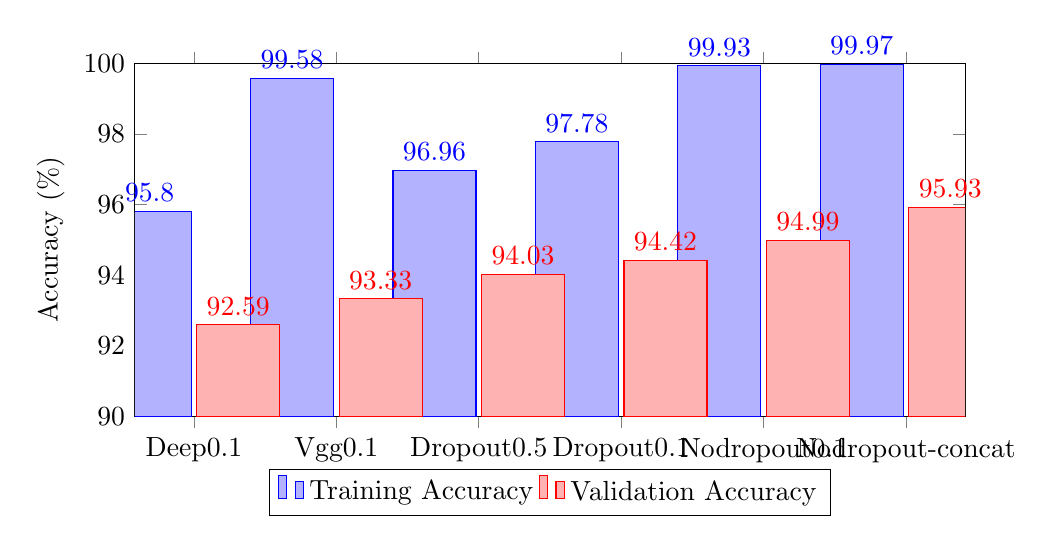
\begin{tikzpicture}
        \begin{axis}[
            ybar,
            symbolic x coords={Deep0.1, Vgg0.1, Dropout0.5, Dropout0.1, Nodropout0.1, Nodropout-concat},
            xtick=data,
            nodes near coords,
            ymin=0,
            ylabel={Accuracy (\%)},
            xlabel={Model},
            width=1.0\textwidth,
            height=0.5\textwidth,
            bar width=30pt,
            enlarge x limits={abs=0.75cm},
            ymin=90, ymax=100,
            legend style={at={(0.5,-0.15)}, anchor=north, legend columns=-1},
            ]
            \addplot coordinates {(Deep0.1, 95.80) (Vgg0.1, 99.58) (Dropout0.5, 96.96) (Dropout0.1, 97.78)  (Nodropout0.1, 99.93) (Nodropout-concat, 99.97)};
            \addplot coordinates {(Deep0.1, 92.59) (Vgg0.1, 93.33) (Dropout0.5, 94.03) (Dropout0.1, 94.42)   (Nodropout0.1, 94.99) (Nodropout-concat, 95.93)};
            \legend{Training Accuracy, Validation Accuracy}
        \end{axis}
    \end{tikzpicture}
    \caption{Comparison of Model Architectures}
    \label{fig:model_comparison}
\end{figure}
\paragraph{Settings}
The similarity between these models are convolution layers. Basically, we utilize \texttt{channels=64} and \texttt{channels=128}. Except for Vgg net, we utilize Resnet configuration, with "same" paddings. Also, we add a Maxpooling after each individual convolution layer(but not after residual layers.) Thus we could extract each range of features in the photo(similar to DenseNet). A Batch Normalization is added after each layer. Activation layers varies from SiLU, GELU, LeakyReLU (but does not affect the result a lot).
\paragraph{Unsuccessful Tries -- MoE} At the beginning, I tries to utilize MoE architecture to train the model. However, We mainly faces the following questions:
\begin{itemize}
    \item Total Model size is limited by 5M, thus each expert's size is limited, leading to a poor performance.
    \item Classification tasks is not suitable for MoE, MoE has its advantage for a faster inference speed and tasks that could be seperated to different experts. Leading to a better performance in regression tasks.
    \item Need a extra gate to determine which expert to use, leading to a slower training speed.
\end{itemize}
\paragraph{Conclusion}
After implementing this coding project, some experience is gained:
\begin{itemize}
    \item Architecture is important, especially need to be carefully chosen for a specific task and a limited model size.
    \item Data Augmentation is also important, but should not be setted too hard, in case of the poor ability of model to converge.
    \item The model's size is limited, thus the model's width also means much.
    \item Some tricks (such as no dropout after BatchNorm, etc.) should be considered.
    \item for a model that is not deep enough, residual connection does not have a significant improvement. However, it indeed increase the model's performance, and make the training progress more stable.
    \item concatenation for last several layers are essential, making the model extract each range of features in the photo.
\end{itemize}
Afterall, the model's best performance on valid set is \textbf{95.93\%}.
\end{document} 
